%%%%%%%%%%%%%%%%%%%%%%%%%%%%%%%%%%%%%%%%%%%%%%%%%%%%%%%%%%%%%%%%%%%%%%%%%%%%%%%%
%2345678901234567890123456789012345678901234567890123456789012345678901234567890
%        1         2         3         4         5         6         7         8

\documentclass[letterpaper, 10 pt, conference]{ieeeconf}  % Comment this line out
                                                          % if you need a4paper
%\documentclass[a4paper, 10pt, conference]{ieeeconf}      % Use this line for a4
                                                          % paper

\IEEEoverridecommandlockouts                              % This command is only
                                                          % needed if you want to
                                                          % use the \thanks command
\overrideIEEEmargins
\usepackage{url}
\usepackage{graphicx}
\usepackage{caption}

% See the \addtolength command later in the file to balance the column lengths
% on the last page of the document



% The following packages can be found on http:\\www.ctan.org
%\usepackage{graphics} % for pdf, bitmapped graphics files
%\usepackage{epsfig} % for postscript graphics files
%\usepackage{mathptmx} % assumes new font selection scheme installed
%\usepackage{times} % assumes new font selection scheme installed
%\usepackage{amsmath} % assumes amsmath package installed
%\usepackage{amssymb}  % assumes amsmath package installed

\title{\LARGE \bf
Effects of Containerization on Network Performance
}

%\author{ \parbox{3 in}{\centering Huibert Kwakernaak*
%         \thanks{*Use the $\backslash$thanks command to put information here}\\
%         Faculty of Electrical Engineering, Mathematics and Computer Science\\
%         University of Twente\\
%         7500 AE Enschede, The Netherlands\\
%         {\tt\small h.kwakernaak@autsubmit.com}}
%         \hspace*{ 0.5 in}
%         \parbox{3 in}{ \centering Pradeep Misra**
%         \thanks{**The footnote marks may be inserted manually}\\
%        Department of Electrical Engineering \\
%         Wright State University\\
%         Dayton, OH 45435, USA\\
%         {\tt\small pmisra@cs.wright.edu}}
%}

\author{Swathi Hoysala, Jeyavaishnavi Muralikumar, Ashrith Sheshan % <-this % stops a space
}


\begin{document}



\maketitle
\thispagestyle{empty}
\pagestyle{empty}


%%%%%%%%%%%%%%%%%%%%%%%%%%%%%%%%%%%%%%%%%%%%%%%%%%%%%%%%%%%%%%%%%%%%%%%%%%%%%%%%


%%%%%%%%%%%%%%%%%%%%%%%%%%%%%%%%%%%%%%%%%%%%%%%%%%%%%%%%%%%%%%%%%%%%%%%%%%%%%%%%
\section{REVIEW}

The stated goal of this project was to measure networking performance in container environments. Our initial plan was to focus our evaluation in the following directions:

\begin{enumerate}
	\item Do conclusions based on the evaluation of LXC \cite{zhao2017performance} necessarily generalize to different container images?
    \item What overhead does containerization introduce on top of virtualization?
    \item Does the network performance of containers depend on the underlying OS of the host?
\end{enumerate}

In our previous update, we noted that TCP performance was comparable whereas UDP performance improved due to increased CPU utilization. 

\section{EXPERIMENTAL SETUP}

The experiments reported in this checkpoint were run on the provided setup, which is identical VMs with 4-cores @ 2.83 GHz and 16 GiB of memory. We're not sure of the network between our VMs, but it shouldn't matter since we are measuring overheads anyway. Unless otherwise mentioned, the container image used was ubuntu-17.10. The container platform used was Docker version 17.12.0-ce.

\section{CURRENT RESULTS}

\subsection{ICMP overhead}

We checked how ping works VM-to-VM and in the container-to-VM setup and noticed the following values.

\vspace{5pt}

\begin{tabular}{|p{75pt}|p{25pt}|p{25pt}|p{25pt}|p{25pt}|}
\hline
Scenario & RTT avg	& RTT min & RTT max	& RTT sdev \\
\hline
VM to VM &	0.095  & 0.099 & 0.136 & 0.018  \\
\hline
Container to VM	& 0.123 & 0.144 & 0.224 & 0.028 \\
\hline
\end{tabular}
\captionof{table}{ICMP RTT stats; All values are in ms}

\vspace{5pt}

All values are in milliseconds. We can see a rough 25\% overhead in RTT, which we believe is due to an extra hop caused by the containerization. This is because the per hop latency is pretty much constant in both setups, as we will show later.

\subsection{TCP and UDP bandwidth}

We tried to compare the TCP and UDP bandwidth for both setups, i.e., between the VMs in one case, and by sending requests from a container on one of those VMs to the other in the second case. We used qperf \cite{qperf} version 0.4.9 to obtain the following measurements in the latter case.

\vspace{5pt}

\begin{tabular}{|p{25pt}|p{30pt}|p{30pt}|p{40pt}|p{40pt}|}
\hline
Image & TCP bw & UDP bw & TCP cpu usage & UDP cpu usage \\
\hline
centos & 118 MB/s & 213 MB/s & 10.8\% & 100\% \\
\hline
ubuntu & 118 MB/s & 220 MB/s & 11.3\% & 100\% \\
\hline
\end{tabular}
\captionof{table}{Bandwidth measurement from qperf on a container to a VM for packet size 2 KB}

\vspace{10pt}

The figures reported above are for packet size 2 KB. We found, surprisingly that the TCP bandwidth was pretty much constant with varying packet size, whereas the UDP bandwidth increased. We believe that the qperf results may be normalized for some reasons, but are not sure about the reason for this behavior. Summing up the bandwidth results, we find that:

\begin{itemize}
\item UDP bandwidth measurement inside a container causes 100\% cpu usage, leading to higher observed bandwidth than with VM-to-VM communication. This is not an artifact of using qperf, because we observed similar results while using other tools such as netperf \cite{netperf}. This does not happen with TCP bandwidth measurement.
\item TCP bandwidth does not seem to increase inside a container as it should with increasing packet size, whereas UDP bandwidth does (see figure). A possible explanation is that we are not using large enough packet sizes. However, we observed using our own scripts that bandwidth increase for TCP is slow for the VM-to-VM case also. We do not have an explanation at this point.
\end{itemize}

\begin{figure}[h]
	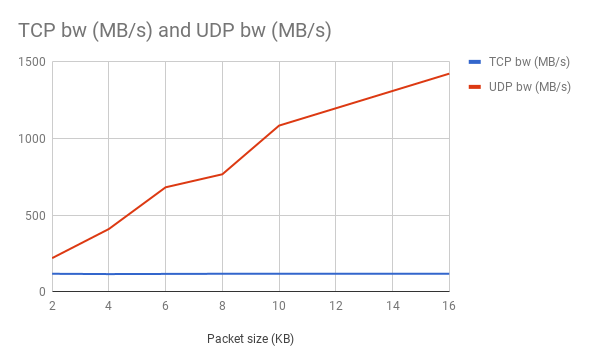
\includegraphics[width=0.5\textwidth]{chart.png}
    \caption{TCP and UDP bandwidth w.r.t packet size, measured by sending data from a container image to another VM using qperf}
\end{figure}

TCP bandwidth is comparable to the VM-to-VM case whereas UDP bandwidth is significantly higher due to the high cpu usage. We plan to repeat this experiment with our own scripts to better understand what's happening.

\subsection{TCP RTT}

Since qperf by construction reports per hop latency, we measure TCP overhead by writing our own script to measure RTT between the two hosts. As for every other experiment, we have two setups: VM-to-VM and container-to-VM. We averaged the results over multiple round trip communications. As can be seen from the following table, the overhead was about 10\%.

\vspace{5pt}

\begin{tabular}{|p{80pt}|p{55pt}|p{55pt}|}
	\hline
	Scenario & Mean RTT & Std dev \\
    \hline
    VM to VM & 235.289 & 20.2013 \\
    \hline
    VM to container & 259.1474 & 28.2726 \\
	\hline
\end{tabular}
\captionof{table}{TCP RTT; All values are in microseconds}

\vspace{5pt}

\section{PLAN}

Since we've been running into issues due to our lack of understanding on how network measurement tools work, we plan to conduct the rest of the experiments with our own scripts. Over the next couple of weeks, this is what we plan to do:

\begin{itemize}
\item Look at TCP and UDP bandwidth in the container and compare with VM-to-VM communication, as well as try to figure out why UDP throughput is so high in containers.
\item Measure UDP performance overheads (RTT) in container environments.
\item Measure performance impact in multi container environments, where multiple containers share a host. We expect degradation due to contention for the docker0 network interface.
\item Measure performance impact in multi-flow traffic. Similar to the multi container setup, we will have multiple flows being routed through the docker0 interface.
\item Measure overheads in multiple host environments, and see if they compare.
\end{itemize}


\addtolength{\textheight}{-12cm}   % This command serves to balance the column lengths
                                  % on the last page of the document manually. It shortens
                                  % the textheight of the last page by a suitable amount.
                                  % This command does not take effect until the next page
                                  % so it should come on the page before the last. Make
                                  % sure that you do not shorten the textheight too much.

%%%%%%%%%%%%%%%%%%%%%%%%%%%%%%%%%%%%%%%%%%%%%%%%%%%%%%%%%%%%%%%%%%%%%%%%%%%%%%%%



%%%%%%%%%%%%%%%%%%%%%%%%%%%%%%%%%%%%%%%%%%%%%%%%%%%%%%%%%%%%%%%%%%%%%%%%%%%%%%%%



%%%%%%%%%%%%%%%%%%%%%%%%%%%%%%%%%%%%%%%%%%%%%%%%%%%%%%%%%%%%%%%%%%%%%%%%%%%%%%%%

%%%%%%%%%%%%%%%%%%%%%%%%%%%%%%%%%%%%%%%%%%%%%%%%%%%%%%%%%%%%%%%%%%%%%%%%%%%%%%%%

\bibliographystyle{plain}
\bibliography{references.bib}

\end{document}
